\documentclass[aspectratio=169]{beamer}
\usepackage[utf8]{inputenc}

\setbeamersize{text margin left=3mm,text margin right=3mm} 

\usetheme{Oxygen}
\usepackage{graphicx}
\usepackage{hyperref}
%\usepackage{movie15}
\usepackage{textpos}
\usepackage{fancybox}
\usepackage{colortbl}
\usepackage{rotating}
%\usepackage{subfigure}
\usepackage{subcaption}
\usepackage{multicol}
\usepackage{multirow}
\usepackage{amsmath,amssymb,amsfonts,amsbsy,dsfont}
\usepackage{mathrsfs}
\usepackage{amsthm}
\usepackage{bm}
\usepackage{array}
%\usepackage[caption=false]{subfig}
\usepackage{arydshln}


\newcommand{\x}{\negthinspace\times\negthinspace}
\usepackage{etoolbox}

\usepackage[nopar]{lipsum} 

\newif\ifcomment
\newcommand{\Com}{\par\footnotesize\itshape\commenttrue}

\newenvironment{Itemize}
 {%
  \edef\Itemizecurrent{\the\font}%
  \itemize
  \preto{\item}{\ifcomment\par\Itemizecurrent\fi}%
 }{%
  \enditemize
 }


%%%%%%%%%%%%%%%%%%%%%%%%%%%%%%%%%%%%%%%%%%%%%%%%%%%%%%
%%%%%%%


\title[A Deep Learning Approach for Image-based Semantic Segmentation with Preserved Interpretability]{A Deep Learning Approach for Image-based Semantic Segmentation with Preserved Interpretability}
\author{\normalsize{Juan Carlos Aguirre Arango}\\ \scriptsize{jucaguirrear@unal.edu.co}}
\institute{
\includegraphics[width=0.15\textwidth]{EscudoUN.png}\\\footnotesize{
Universidad Nacional de Colombia \\ Signal Processing and Recognition Group - SPRG
\\
Advisor: Andrés Marino Álvarez Meza, Ph.D.\\

}}
\date[]{\scriptsize{\today}}
%%-------------------------------------------------------------------
%% Options
%%-------------------------------------------------------------------
\setbeamercovered{dynamic}
\setbeamertemplate{navigation symbols}{}



\begin{document}

{\setbeamertemplate{headline}{}
\setbeamertemplate{footline}{}
\begin{frame}{}
\vspace{-0.7cm}
    \titlepage 
\end{frame}
}


\frame
{ \frametitle{Outline}
{\small 
  \tableofcontents[]}
}

\AtBeginSection[]
{
  \begin{frame}
  \frametitle{Outline}
  \tableofcontents[currentsection]
  \end{frame}
}



%%%%%%%%%%%%%%%%%%%%%%%%%%%%%%%%%%%%%%%%%
\section[Motivation]{Motivation}

\begin{frame}{Frame Title}
    \lipsum
\end{frame}



\section{Problem Statement}

\begin{frame}{Title}
    \lipsum
\end{frame}

\section{State of the Art}

\begin{frame}{Frame Title}
\begin{figure}
    \centering
    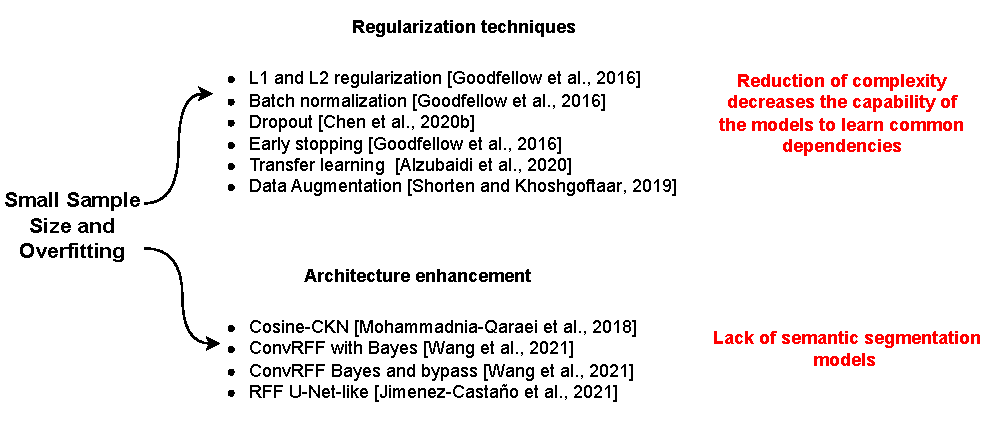
\includegraphics[width=0.8\linewidth]{Figures/State-of-the-arr-obj1.pdf}
    %\caption{Caption}
    %\label{fig:my_label}
\end{figure}    
\end{frame}

\begin{frame}{Frame Title}
\begin{figure}
    \centering
    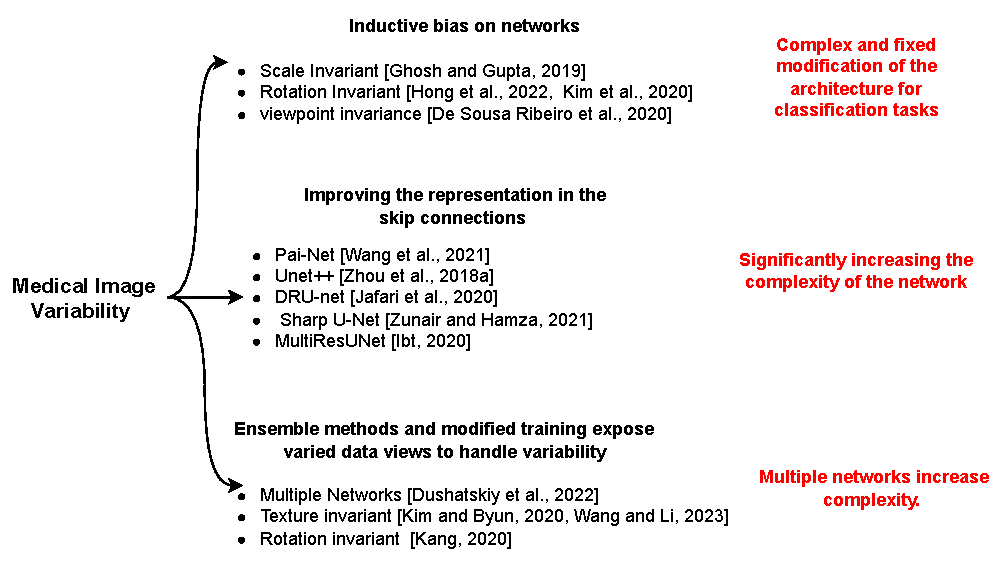
\includegraphics[width=0.8\linewidth]{Figures/State-of-the-ar-obj2.pdf}
    %\caption{Caption}
    %\label{fig:my_label}
\end{figure}    
\end{frame}


\begin{frame}{Frame Title}
\begin{figure}
    \centering
    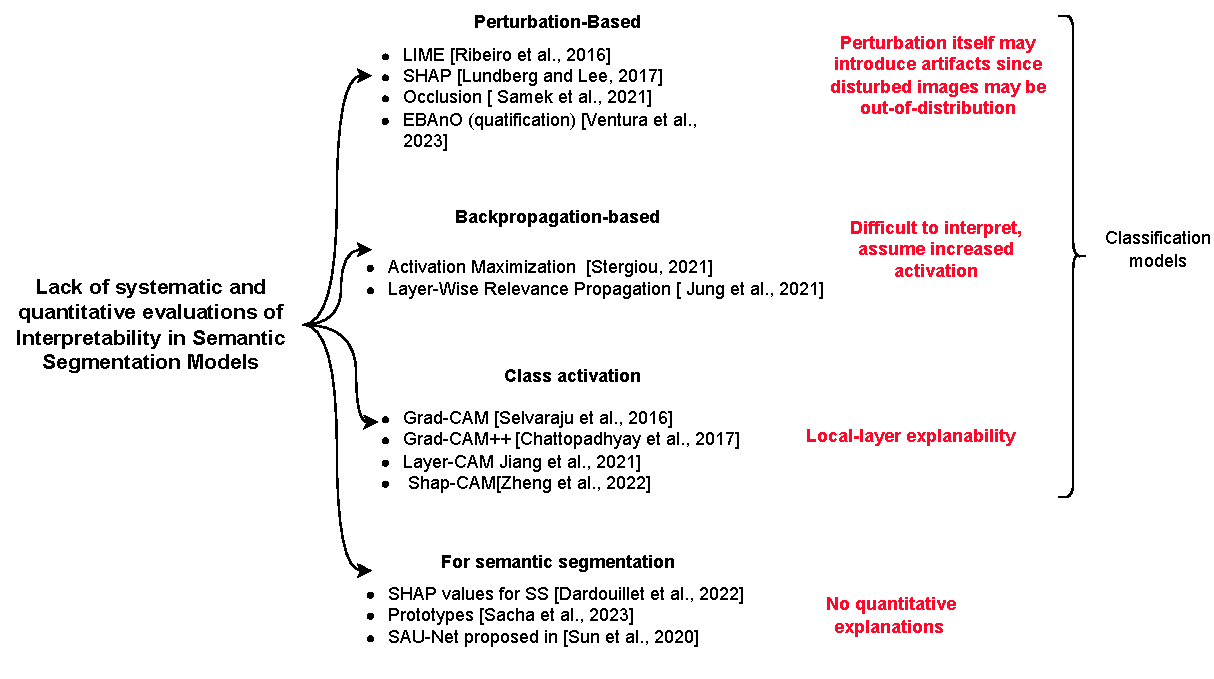
\includegraphics[width=0.8\linewidth]{Figures/State-of-the-ar-obj3.pdf}
    %\caption{Caption}
    %\label{fig:my_label}
\end{figure}    
\end{frame}



\section{Aims}

\begin{frame}{General Aim}
    Develop a DL-based semantic image-segmentation methodology incorporating a convolutional layer based on RFF, and comprehensive interpretability measures to encode relevant patterns related to the structures of interest and improve generalization performance under conditions of scarce data in shallow network architectures.
\end{frame}

\begin{frame}{Specific Aims}
     \begin{itemize}

        \item To design an extension of RFF for spatial data with optimization through gradient descent for Generalization under scarcity data through local and equivariant characterization for shallow network architectures.

        \item To develop a Semantic Segmentation approach based on type encoder-decoder architectures that incorporate Random Fourier Features for enhanced skip representation in shallow networks for improved capture of small and variable objects in semantic segmentation tasks.


        \item To develop a post-hoc interpretability approach based on Measures for quantitative assessment of relevance maps taking into account the spatial information of Semantic Segmentation task for global and layer-wise interpretability

    \end{itemize}

\end{frame}


\section{Methodology}

\begin{frame}{Methodology}
    \begin{figure}
        \centering
        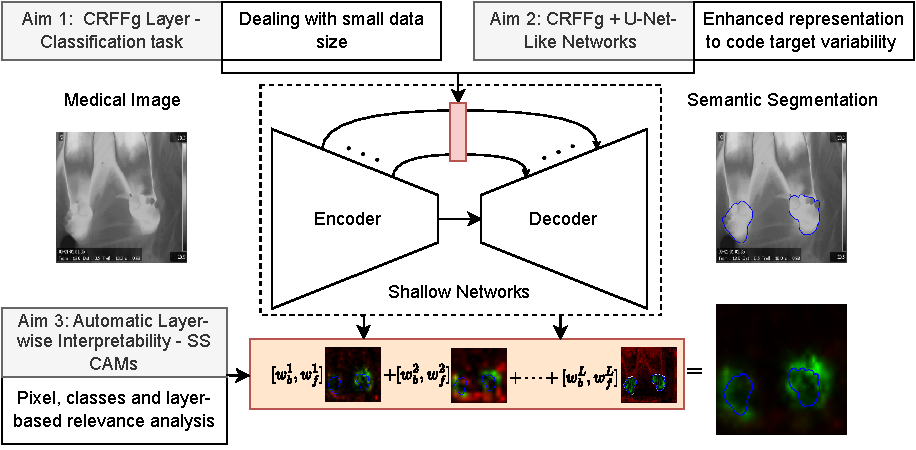
\includegraphics[width=0.9\linewidth]{Figures/contribution_thesis.pdf}
        %\caption{Caption}
        %\label{fig:my_label}
    \end{figure}
\end{frame}


\section{Experimental Set-up}

\section{Comparative Results}

\section{Conclusions}

\begin{frame}{Conclusions}
    
\end{frame}

\begin{frame}{Future Work}
    
\end{frame}

\begin{frame}{Academic Discussion}
    
\end{frame}


\begin{frame}{Acknowledgments}

\begin{itemize}
    \item \textit{``Herramienta de apoyo a la predicción de los efectos de anestésicos locales vía neuroaxial epidural a partir de termografía por infrarrojo" (Code 111984468021)} funded by MINCIENCIAS
    \item \textit{``Sistema prototipo de visión por computador utilizando aprendizaje profundo como soporte al monitoreo de zonas urbanas desde unidades aéreas no tripuladas" (Hermes Code 55261)}, funded by Universidad Nacional de Colombia.
\end{itemize}



\begin{center}
	{\large{\textbf{\textcolor[rgb]{0.00,0.00,1.00}{Thank you!}}}}\\
	\vspace{0.1cm}
	 Juan Carlos Aguirre Arango\\ \scriptsize{jucaguirrear@unal.edu.co}
\end{center}    
    
\end{frame}


\section{References}


\begin{frame}[allowframebreaks]
\frametitle{References}
{\tiny 
\bibliographystyle{apalike}
\bibliography{References}
}
\end{frame}




\end{document}

